
\chapter{Analysis and High-Level Design}

It is the goal of this thesis to enable detection of sleep-related illnesses 
with the aid of an Android device and low-cost sensors, and to further analyze 
and evaluate sleep- and breath-related patterns. We developed an application, 
called \textit{Nidra}, which attempts to collect, analyze and share data collected 
from external sensors, all on a mobile device. Also, Nidra acts as a platform for 
modules to enrich the data, thus extending the functionality of the application.

The motivation behind this application is to provide an interface for patients 
to potentially run a self-diagnostic (of the illness?) from home, and to aid 
researchers and doctors with analysis of sleep- and breathing-related illnesses 
(e.g., Obstructive Sleep Apnea). An overview of the Nidra application pipeline 
can be found in figure x, beginning with data acquired from a sensor, and ending 
with the data in the Nidra application. As for now, Nidra consists of three 
main functionalities, each related to the requirements defined in Section [Problem Statement]. 

\begin{enumerate}
    \item The application should provide an interface for the patient to 1) record physiological signals (i.e., during sleep); 2) present the results; and 3) export/import the results.
    \item The application should provide an interface for the developers to create modules to enrich the data from records or extend the functionality of the application. 
    \item The application should ensure a seamless and continuous data stream, uninterrupted from sensor disconnections and human disruptions.
\end{enumerate}

This chapter will give a detailed look at the design of Nidra...

\section{Requirement Analysis}

\subsection{Stakeholders}
A stakeholder is a term coined to describe those persons or organizations that have, or claim an interest in the project. Identifying stakeholders is essential to fulfilling the requirement set in the thesis, as they contribute to form and sculpture the application. As discussed by McGrath \textit{et al}. \cite{stakeholderdefined}, stakeholders can be distinguish  into four categories: 1) \textit{contributing (primary) stakeholders} are those that participate in developing and sustaining the project; 2) \textit{observer (secondary) stakeholder} are those who affect or influence the project;  3) \textit{end-user (tertiary stakeholder)} is the one who interact and uses the output of the application; and 4) \textit{invested stakeholder} is one who has control of the project. In Nidra, we have three stakeholders who affect the application, and each can be categorized respectfully.
\begin{itemize}
    \item \textbf{Patients} - are identified as an end-user; they interact with the application.  
    \item \textbf{Researchers/Doctors} - are identified as an observer stakeholder; they might not use the application itself. However, they might use the data obtained from the patients' recordings for further analysis. Additionally, request functionality in the application.
    \item \textbf{Developers} - are identified as a contributor stakeholder; they maintain the application from bugs or extend the functionally of the application. Additionally, they can contribute to developing modules that extend the functionality of the application. 
\end{itemize}

%\subsection{System Requirements}

\subsection{Resource Efficiency}
The application is designed for the use on a mobile device; modern mobile devices are empowered with multi-core processors, a sufficient amount of ROM, and a variety of sensors. However, the battery capacity is restrictive and based on usage. The device may only last for one day before a charge, due to the size of the battery capacity \cite{androidbattery}. The average capacity of a mobile device is around 2000 mAh on budget devices and around 3000 mAh on high-end devices \cite{androidbatteryavg}. The application should be able to run at least 7 hours without any power supply. Also, the device should be capable of handling various sensor connections simultaneously. Therefore, the application should be designed to be resource efficient, by ... 

\subsection{Security and Privacy}
The proposed use of the application is to monitor the sleeping patterns of a user. The application manages and stores personal-data and health-related data about the user on the device. As a consequence, the application should incorporate the CIA triad, which stresses data confidentiality, integrity, and availability \cite{cia}. Any unauthorized access to the data, data leaks, and confidentiality should be appropriately managed on the device. Sharing the data across application or with other users should be granted with the consent from the user.  Besides, a mobile device can be connected to the Internet, which makes it vulnerable to attacks. Also, installed application on the device can manipulate the access to the data. Therefore, revising the security policy defined by Android \cite{androidsecurity} should be contemplated. 

\section{High-Level Design}

\subsection{Task Analysis}
Task analysis is a methodology to facilitate the design of complex systems. Hierarchical task analysis (HTA) is an underlying technique that analyzes and decomposes complex tasks such as planning, diagnosis, and decision making, into specific subtasks \cite{ta}. In Figure \ref{fig:hta_overview} an illustration of the the main components of the project is presented. These components are integral to the development of the project, and in this Section, we will be analyzing system tasks and user-related tasks.

\begin{figure}
    \centering
    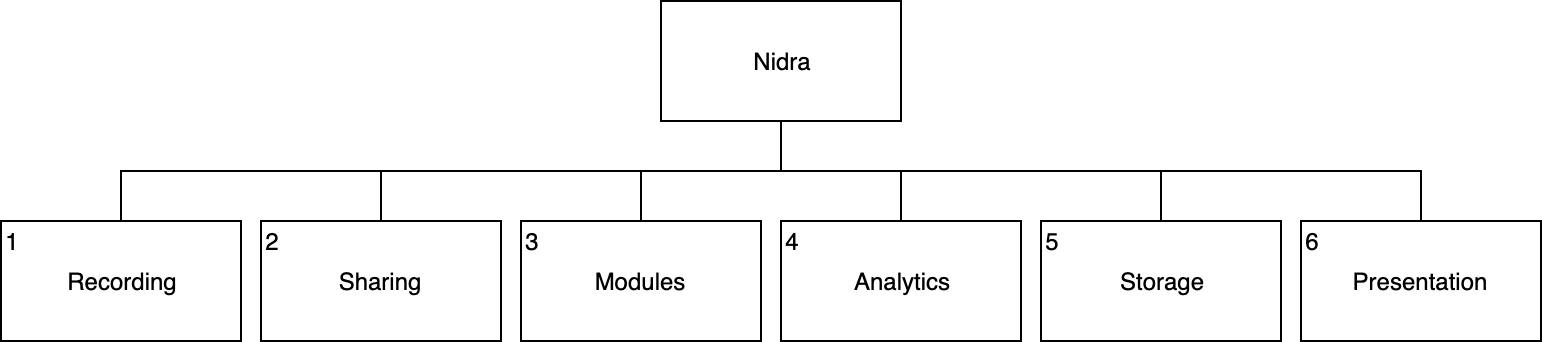
\includegraphics[scale=0.23]{images/TA.png}
    \caption{Recording}
    \label{fig:hta_overview}
\end{figure}

%\subsubsection{System Tasks}

\noindent\textbf{Recording}

\noindent A \textit{recording} is a process of collecting and storing physiological signals (e.g., breathing data) from sensors over an extended period (e.g., overnight). To enable a recording, we need to establish connections to available sensors, collect samples from the sensors, and store the samples on the device. A \textit{sensor} is a device that transforms analog signals from the real world into digital signals. The digital signals are transmittable over Link Layer technologies (e.g., BlueTooth), and the communication between a sensor and device occurs based on the protocols the sensor supports. A \textit{sample} is a single sensor reading containing data and metadata, such as time and the physiological data. During the recording session, ensuring that the sensors and the devices maintain connectivity such that the record contains meaningful data.  Once a recording session has terminated, a \textit{record} with metadata about the recording session is stored, alongside the samples.    

\noindent \textbf{Sharing}

\noindent Sharing is a mechanism to export and import records across applications. \textit{Exporting} consists of bundling one or more records with correlated samples into a transmittable format and transferring the bundled records over a media (e.g., mail). \textit{Importing}, on the other hand, consists of locating the bundled records on the device, parsing the content and storing it on the device. The sharing mechanism allows the patients to send their records to researchers/doctors.

\noindent \textbf{Module}

\noindent A \textit{module} is an independent application that is installed and launched in Nidra (hereafter: application), to provide extended functionality and data enrichment. A module does not necessarily interact with the application. However, it utilizes the data (e.g., records). For example, a module could be using the records to feed a machine-learning algorithm to predict obstructive sleep apnea. Installing a module is achieved by locating the module-application on the device, and storing the reference in the application. Due to limitations in Android, the module-application cannot be executed within the application. Therefore, the module-application is a standalone Android application. Furthermore, the development of the module-application is independent of the application. 

\noindent \textbf{Analytics}

\noindent Analytics is the visualization and interpretation of patterns in the records. The application facilitates the recording of breathing data, which enables the detection and analysis of sleep-related breathing disorder. There are various analytical methods, ranging from graphs to advanced machine learning algorithms, and incorporating a simple time series plot can indirectly aid in the analysis. For example, plotting a time series graph where the breathing data are on the Y-axis and the time on X-axis, provides a graphical representation of the data that can be further analyzed within the application.

\noindent \textbf{Storage}

\noindent Storage is the objective of achieving persistent data; data remain available after application termination. To enable storage, we use a database for a collection of related data that is easily accessed, managed, and updated. The database should be able to store records, samples, modules, and biometrical data related to the user (i.e., gender, age, height, and weight). Structuring a database that is reliable, efficient, and secure is a crucial part of achieving persistent storage. Android provides several options to enable storage on the device (e.g., internal storage and database).

\noindent \textbf{Presentation}

\noindent Presentation is the concept of exhibiting the functionality of the application to the user. A user interface (UI) is the part of the system that facilitates interaction between the user and the system. In Nidra, determining the screen layout, color palette, interactions, and feedback on actions is part of the development of a user interface. 

\section{Seperation of Concerns}
Separation of concern is a paradigm that classifies an application into concerns at a conceptual and implementational level. It is beneficial for reducing complexity, improving understandability, and increasing reusability \cite{soc}. The concerns in this thesis are the individual tasks defined in task analysis. Each concern is conceptualized with a graph of components, the functionality of each component when combined constitutes a structure. The structure of each concern is derived based on research and development. 


\subsection{Recording}
There are several approaches to assemble components to achieve a recording, and we review an alternative structure. In Figure \ref{fig:hta_recording} we have an HTA graph, which illustrate the building blocks to enable a recording and their dependencies:

\begin{figure}
    \centering
    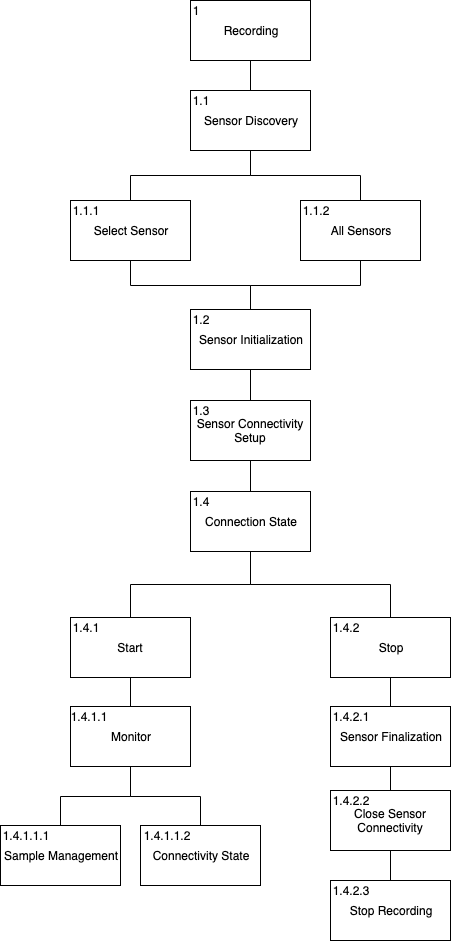
\includegraphics[width=0.65\textwidth]{images/Recording.png}
    \caption{Recording}
    \label{fig:hta_recording}
\end{figure}

\begin{itemize}
    \item Sensor Discover: Has to find all eligible sensors that can enable a recording.
    \item Select Sensors: From the sensor discovery, we can choose preferable sensors sources.
    \item  All Sensors: More straightforward, we sample from all of the available sensors.
    \item Sensor Initialization: Once we have a list of sensors sources, we need to establish and initialize a connection with the sensors. Occasionally a sensor might use some time to connect, or unforeseen occurrence is hindering the initialization of the sensor. Thus, blocking the state of the recording. 
    \item Sensor Connectivity Setup: Additionally, we establish a connection between the application and the sensor source. All data exchange occurs over the established interface. 
    \item Connection Stat: Based on sensors establishments we can proceed to either start or stop a recording. 
    \item Start: By starting, we notify the sensors to begin collecting data, and the view should display that a recording has begun accordingly.
    \item Monitor: Is continuously waiting for new samples to arrive on the interface defined between the application and the sensors.
    \item Sample Management: Once a new sample has arrived, we need to store the sample on a persistent storage.
    \item Connectivity State: If it is an external sensor, the sensor source might disconnect during a recording. Thus, implementing a mechanism to check for continuous data stream is a critical task.
    \item Stop: By stopping, we notify the sensors to stop collecting data from the sensor source.
    \item Sensor Finalization: We notify the sensor to stop sampling data, and close establishment.
    \item Close Sensor Connectivity: We close the interface establishment between the application and the sensors. 
    \item Stop Recording: Once the sensors has closed its connections, we can add additional information to the recording (e.g., title, description, rating). In the end, the recording has concluded and its stored on the mobile device.

\end{itemize}

This suggested structure of a recording is one alternative to enable a recording. Most of the components suggested in the structure are essential to a recording. A naive solution would be to ignore the connectivity state component, by assuming the sensors are connected indefinitely. In our thesis, we will be following 


\subsection{Sharing}

\subsection{Modules}

\subsection{Storage}

\subsection{Presentation}


\section{Data Structure}

\subsection{Data Formats}

The data format is a part of the process of serialization, which enables data storage in a file, transmittal over the Internet, and reconstruction in a different environment. Serialization is the process of converting the state of an object into a stream of bytes, which later can be deserialized by rebuilding the stream of bytes to the original object. There are several data serialization formats; however, JavaScript Object Notation (JSON) and eXtensible Markup Language (XML) are the two most common data serialization formats. In this Section, we will discuss these formats. In the end, we will compare them and choose the format that meets the criteria of being compact, human-readable, and universal. 

\subsubsection{JSON}
JSON or JavaScript Object Notation is a light-weight and human-readable format that is commonly used for interchanging data on the web. The format is a text-based solution where the data structure is built on two structures: a collection of name-value pairs (known as objects) and ordered list of values (known as arrays). The JSON format is language-independent and the data structure universally recognized \cite{jsonorg, jsonvxml}. However, it is limited to a few predefined data types (i.e., string, number, boolean, object, array, and null), and extending the data type has to be done with the preliminary types. 

\begin{lstlisting}[language=json, caption={My Caption}, captionpos=b]
{
    "user": {
        "firstname": "Ola"
        "lastname": "Nordmann"
    }
}
\end{lstlisting}

\subsubsection{XML}
XML or eXtensible Markup Language is a simple and flexible format derived from Standard Generalized Markup Language (SGML), developed by the XML Working Group under the World Wide Web Consortium (W3C). An XML document consists of markups called tags, which are containers that describe and organize the enclosed data. The tag starts with \verb|<| and ends with \verb|>|; the content is placed between an opening tag and a closing tag (see listing). \cite{w3xml, jsonvxml} XML provides mechanisms to define custom data types, using existing data types as a starting point, making it extensible for future data. 

\begin{lstlisting}[language=json, caption={My Caption}, captionpos=b]
<user>
    <firstname>Ola</firstname>
    <lastname>Nordmann</lastname>
</user>
\end{lstlisting}

\subsubsection{Comparing}
We will compare JSON and XML features and performance with the study conducted by Saurabh and D’Souza \cite{jsonvxml}. There are apparent differences in the two data formats which affect the overall readability, extensibility, bandwidth performance, and ease of mapping. XML documents are easy to read, while JSON is obscure due to the parenthesis delimiters. XML allows for extended data types, while JSON is limited to a few data types. XML takes more bandwidth due to the metadata overhead, while JSON data is compact and use less amount of bandwidth.

Moreover, a few benchmarks were conducted to measure memory footprint and parsing runtime when serializing and deserializing JSON and XML data. From the conclusion,  in terms of memory footprint and parsing runtime, JSON performances better than XML but at the cost of readability and flexibility. While these format structures are applicable for transmitting data, choosing a format that is compact, human-readable, and a standard format that is extensible and scalable for future data is essential. In our design, we will be using the JSON format for transmission of the data.

\subsection{Data Entities}
Data entities are objects (e.g., things, persons, or places) that the system models and stores information about. Subsection about Storage introduces four data entities in our application (i.e., user, record, sample, and module). In Figure \ref{fig:dataentries}, the relation between the data entities are shown. Record and sample stores information about the recording, and are separated into two individual entities in order to reduce data redundancy and improve data integrity. Although, samples have a reference to its record so they can be associated with each other. A user stores biometrical information related to the user, the user in the application are patients. A record contains the state of the user's biometrical information at the time of the recording. In other words, the user's biometrical information can change over time (e.g.,  weight changes); therefore, capturing the exact biometrical information at the time of the recording is essential in the context of detecting sleeping illnesses with relation to the biometrical information.  A module is independent of the other data entities and stores information about the name and the package name of the module-application. The package name is used to locate and launch the module-application. 

In this Subsection, we will demonstrate the properties of each data entity in Nidra; storage structure of the entities, and illustration of the data structure for each entity.  

\begin{figure}
    \centering
    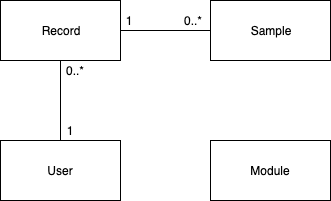
\includegraphics[scale=0.6]{images/DataEntries.png}
    \caption{Modules}
    \label{fig:dataentries}
\end{figure}

\subsubsection{Record}

A record is a table in the database that stores metadata related to the recording session. In Table 4.1, an illustration of the structure of a record is shown, with an entry of dummy data. In Nidra, the fields in the table for a record describe the data that is stored, which is separated into:
\begin{itemize}
	\item \verb|ID|: Unique identification of a record, also a primary key for the entry.
	\item \verb|Name|: A name of the record to easily recognize the recording.
	\item \verb|Description|: A summary over the recording session provided by the user It can be used to briefly describe how the recording session felt (e.g., any abnormalities during the sleep).
	\item \verb|MonitorTime|: The recording session duration in milliseconds.
	\item \verb|Rating|: Giving a rating on how the sleeping session felt, in a range between 0-5. 
	\item \verb|User|: User's biometriocal information encoded into a JSON string format, in order to capture the state of the user at recording. 
	\item \verb|CreatedAt|: Date of creation of the recording in milliseconds (since January 1, 1970, 00:00:00 GMT).
	\item \verb|UpdatedAt|: Date of update of the recording in milliseconds (since January 1, 1970, 00:00:00 GMT).
\end{itemize}


\begin{table}
\begin{center}
\scalebox{0.75}{
\begin{tabular}{ |c|c|c|c|c|c|c|c| } 
\hline
\textbf{id} & \textbf{name} & \textbf{description} & \textbf{monitorTime} & \textbf{rating} & \textbf{user} & \textbf{createdAt} & \textbf{updatedAt} \\
\hline
1 & Record \#1 & - & 5963088 & 2.5 & \{...\} & 1554406256000 & 1554406256000  \\ 
\hline
\end{tabular}}
\caption{Example entry in record table}
\end{center}
\end{table}


\subsubsection{Sample}
A sample is a single sensor reading containing data and metadata related to the recording session. Samples are stored separated from a record; however, they are linked with a field in the table.  In Table 4.1, an illustration of the structure of a sample is shown, with an entry of dummy data. In Nidra, the fields in the table for a sample describe the data that is stored accordingly to the data provided by Flow SweetZpot (ref), which are separated into:
\begin{itemize}
	\item \verb|ID|: Unique identification of a sample, also a primary key for the entry.
	\item \verb|RecordID|: An identification to its correlated record, also a foreign key. 
	\item \verb|ExplicitTS|: Timestamp of sample arrival based on the time in the sensor. 
	\item \verb|ImplicitTS|: Timestamp of sample arrival based on the time on the device. 
	\item \verb|Sample|: Sensor reading contains metadata and data according to Flow Sweetzpot. The sensor aggregates seven samples in a single sensor reading. 
\end{itemize}

\begin{table}
\begin{center}
\scalebox{0.60}{
\begin{tabular}{ |c|c|c|c|c| } 
\hline
\textbf{id} & \textbf{recordId} & \textbf{explicitTS} & \textbf{implicitTS} & \textbf{sample} \\
\hline
1 & 1 & 1554393086000 & 1554400286000 & Time=0ms, deltaT=100, data=1906,1891,1884,1881,1876,1718,1690 \\ 
\hline
\end{tabular}}
\caption{Example entry in sample table}
\end{center}
\end{table}


\subsubsection{Module}
A module is a table in the database that stores all modules installed by the user in the application. In Table 4.3, an illustration of the structure of a module is shown, with an entry of dummy data. In Nidra, the fields in the table contain the name of the module and the reference to the module and can be summarized as: 
\begin{itemize}
    \item \verb|ID|: Unique identification of a module, also a primary key for the entry.
    \item \verb|Name|: The name of the module-application.
    \item \verb|PackageName|: The package name of the module-application, such that it can be launched from Nidra. 
\end{itemize}

\begin{table}
\begin{center}
\scalebox{0.8}{
\begin{tabular}{ |c|c|c| } 
\hline
\textbf{id} & \textbf{name} & \textbf{packageName} \\
\hline
1 & OSA Predicter & com.package.osa\_predicter \\ 
\hline
\end{tabular}}
\caption{Example entry in module table}
\end{center}
\end{table}


\subsubsection{User}
The user of the application is the patient, which provides biometrical data (e.g., weight, height, and age). The biometrical data is part of the application to enrich the record. The record captures the biometrical state of the user at the time of the recording in the context of detecting sleeping illnesses with the relation to the biometrical data. In Nidra, the user entity is not a part of the database, but as an object stored in the device. The design decision of this choice is because the application is limited to one user at the time, and it makes it convenient to capture the state of the object of the given time of recording. It is possible to create a table in the database for the user entity, and for each time the user changes the biometrical data insert it is a separate entry in the database. The record could then have a reference to the latest user entry. However, that increases the complexity of the system, and as of now, the design of the application is to store the user's biometrical data into an object on the device. 

In Listing X, an illustration of the structure of a user is shown, with  dummy data. In Nidra, the user object is structured in a JSON format and contains biometrical data related to the user: 
\begin{itemize}
    \item \verb|Name|: Name of of the patient.
    \item \verb|Age|: Age of the patient.
    \item \verb|Gender|: Gender of the patient.
    \item \verb|Weight|: Weight of the patient in kilograms.
    \item \verb|Height|: Height of the patient in centimeters.
\end{itemize}

\begin{figure}
\begin{lstlisting}[language=json, caption={My Caption}, captionpos=b]
{
    "user": {
        "name": "Ola Nordmann",
        "age": 50,
        "gender": "Male",
        "height": 180,
        "weight: 60
    }
}
\end{lstlisting}
\end{figure}


\subsection{Data Packets}
Data packets are parcels of data that Nidra receives from external applications (e.g., sensor wrappers) or send to other application (e.g., sharing). From the design choice In the Section above, the format of all the desired data should be according to the JSON format.  In this Section.

\subsubsection{Sharing}

In Section (ref), a proposal to the structure of exporting and importing data is discussed. Two of the components (\verb|Parse Formatted Content| and \verb|Format File|) uses JSON to either encode or decode the data. Listing 4.3 illustrate the content of the encoded data from our application to gain a broader understanding of how the data exchange in sharing operates. The attractive attributes from the encoding are the record (ref) and the samples.  A record is an object that contains meta-data with name, number of samples, recording time, creation date, and user information. Samples are an array of objects that contains data, timestamp, and identification to correlated record. 

\begin{figure}
    
\begin{lstlisting}[language=json, caption={My Caption}, captionpos=b]
{
    "record":{  
        "id": 1,
        "name": "Record 1",
        "rating": 2.5,
        "description": "",
        "nrSamples": 6107,
        "monitorTime": 5963088,
        "createdAt": "Apr 4, 2019 9:30:56 PM",
        "updatedAt": "Apr 4, 2019 9:30:56 PM",
        "user": {  
            "age": 50,
            "createdAt": "---",
            "gender": "Male",
            "height": 180,
            "name": "Ola Nordmann",
            "weight": 60
        }
    },
    "samples": [  
        {  
            "explicitTS":"Apr 4, 2019 5:51:26 PM",
            "implicitTS":"Apr 4, 2019 7:51:26 PM",
            "recordId":1,
            "sample":"Time=0ms, deltaT=100, data=1906,1891,1884,1881,1876,1718,1690"
        },
        ...
    ]
}
\end{lstlisting}
\end{figure}

\subsubsection{Sensor Data}
Sensor data is data acquisition through the Data Dispatching (section background). The data format discussed in (section background). 